\documentclass[a4paper, twocolumn]{article}
\usepackage[pdftex, hidelinks,
            pdftitle={Report},
            pdfauthor={Erik S. Vasconcelos Jansson},
            pdfsubject={Report},
            pdfkeywords={report}]{hyperref}

\usepackage{bm}
\usepackage[T1]{fontenc}
\usepackage[utf8]{inputenc}
\usepackage{algorithmic}
\usepackage{algorithm}
\usepackage{amsfonts}
\usepackage{booktabs}
\usepackage{amssymb}
\usepackage{courier}
\usepackage{booktabs}
\usepackage{graphicx}
\usepackage{listings}
\usepackage{mathtools}
\lstset{basicstyle=\footnotesize\ttfamily,
        breakatwhitespace = false,
        breaklines = true,
        keepspaces = true,
        language = C++,
        showspaces = false,
        showstringspaces = false,
        belowcaptionskip = \bigskipamount,
        framerule = 0.80pt,
        frame = tb,
        numbers = left,
        belowskip = \bigskipamount,
        escapeinside={<@}{@>}}

\title{Introduction to Machine Learning \\
       Individual Laboration Report --3--}
\author{{Erik Sven Vasconcelos Jansson} \\
        {\href{mailto:erija578@student.liu.se}
        {\texttt{erija578@student.liu.se}}} \\
        {Linköping University, \, Sweden}}

\begin{document}
    \pagenumbering{arabic}
    \maketitle % Titles...

    \section*{Assignment 1}

        Now that \emph{linear regression} and \emph{cross-validation} have been studied for \emph{regression problems} (involving continuous target variables), the question is how to apply the same concept to \emph{classification problems} (which involve a discrete amount of target variables). Both \emph{Linear Discriminant Analysis (LDA)} and \emph{Logistic Regression} can be used to achieve this, and also to draw \emph{decision boundaries}.

        In this task the goal is to \emph{classify} the \emph{Sex} of \emph{Australian Crabs} by using their \emph{Carapace Length} and \emph{Rear Width} using \emph{LDA} and thereafter plotting the \emph{decision boundary}. Plotting the data gives Figure~\ref{fig:crabs}. As can be seen, a decision boundary seems to exist.

        Firstly, the \emph{linear parameters} $w_0$ and $\bm{w}$ need to be found for each class $k$, essentially creating our \emph{target hypothesis function} for each one of these $k$. Finding these parameters is done with Equations~\ref{eq:lda}, essentially computing the mean $\bm{\hat{\mu}}_k$ for each class $k$ which is used to derive the \emph{covariance matrices} $\Sigma_k$.

        \begin{equation} \label{eq:lda}
        \begin{split}
            \hat{\pi}_k &= \frac{N_k}{N} \\
            \hat{\mu}_k &= \frac{1}{N_k}\sum_{i \in k}{\bm{x}_i} \\
            \Sigma_k &= \frac{1}{N_k}\sum_{i \in k}{(\bm{\hat{\mu}}_k - \bm{x}_i)(\bm{\hat{\mu}}_k - \bm{x}_i)^\intercal} \\
            \hat\Sigma &= \frac{1}{N}\sum_{k \in K}{N_k \Sigma_k} = \sum_{k \in K}{\frac{\mathrm{cov}\,X_k}{|X_k|}}
        \end{split}
        \end{equation}

        \begin{equation} \label{eq:weights}
        \begin{split}
            w_{k} &= -\frac{\bm{\hat\mu}_k^\intercal}{2}\hat\Sigma^{-1}\bm{\hat\mu}_k + \log\hat{\pi}_k \\
            \bm{w}_{k} &= \hat\Sigma^{-1}\bm{\hat\mu}_k
        \end{split}
        \end{equation}

        Finally, computing $\hat{\Sigma}$ is done by using these $\Sigma_k$, which is thereafter used to calculate $w_0$ and $\bm{w},\, \forall k$. Implementation of these formulae in \emph{R} can be found in Listing~\ref{lst:lda} under lines \texttt{15-39} in the \texttt{lda} function. All equations are in \emph{Friedman et al's}~\cite{friedman2009elements} book.

        \begin{equation} \label{eq:discfun}
        \begin{split}
            \delta_k(\bm{x}) &= w_0 + \bm{w}
        \end{split}
        \end{equation}

        Using the \emph{Discriminant Function} in Equation~\ref{eq:discfun} above, one can plot the line through each class $k$. The \emph{decision boundary} is in-between these 2 lines. In lines \texttt{58-61} we calculate the \emph{intercept} and the \emph{slope} of the \emph{decision boundary}, which gives us all the information needed to produce a new Figure~\ref{fig:boundarylda}. The fit seems perfect, exactly as previous Figure~\ref{fig:crabs}.

        \begin{figure}[h!]
            \centering
            \caption{Sex Classifications of Australian Crabs}
            \label{fig:crabs}
            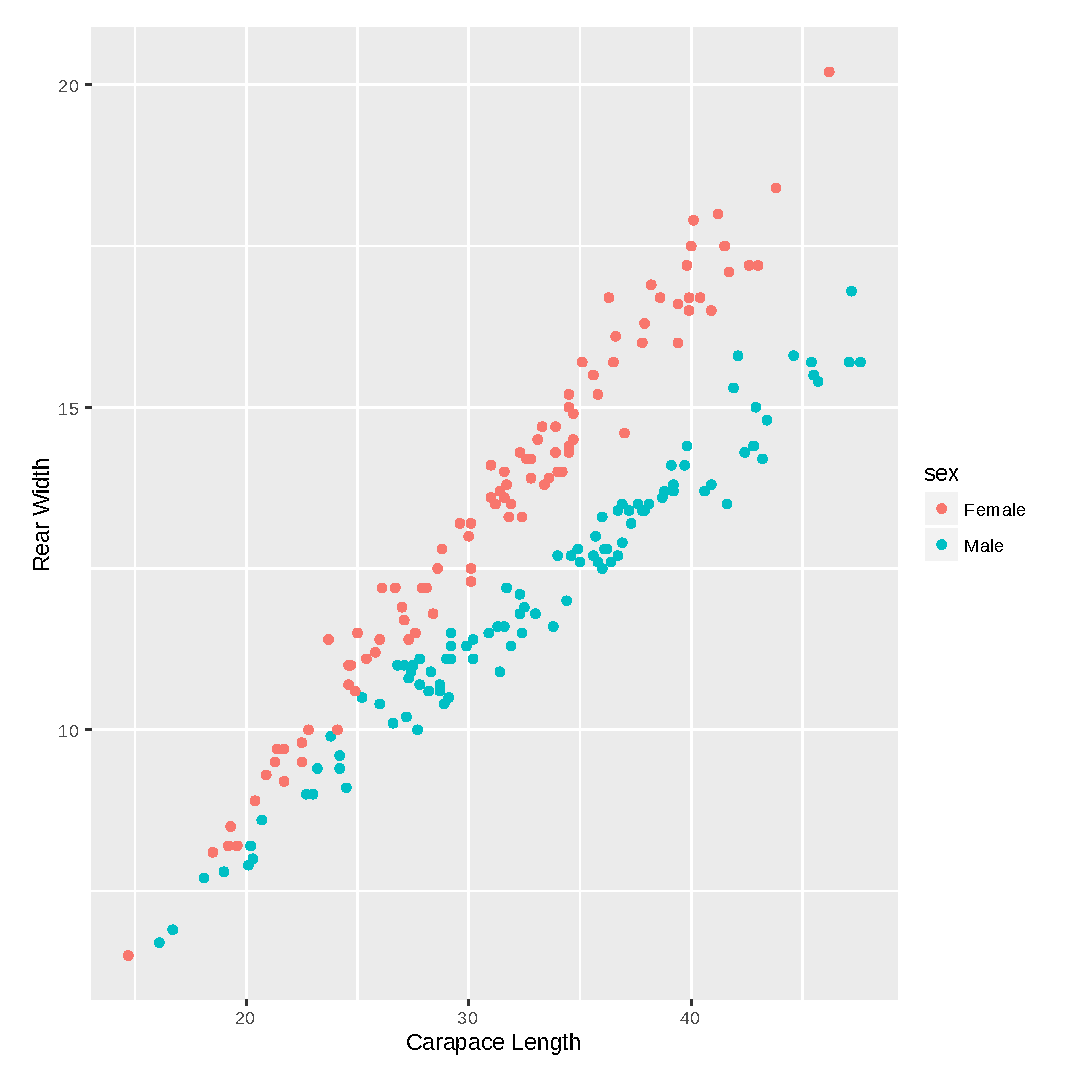
\includegraphics[width=0.45\textwidth]{share/crabs.eps}
        \end{figure}

        \clearpage

        Thereafter, by using \emph{Logistic Regression} instead, Figure~\ref{fig:boundarylr} can be obtained, which misses predictions.

        \begin{table}[h!]
        \begin{center}
        \begin{tabular}{lcc}
            \toprule
                \textbf{Class} & $\bm{w_0}$ & $\bm{w}$ \\
            \midrule
                Female & -22.42 & (-2.161, 8.248) \\
                Male & -12.42 & (-0.213, 2.565) \\
            \bottomrule
        \end{tabular}
        \end{center}
        \caption{Predicted Parameters for Australian Crab}
        \label{table:parameters}
        \end{table}

        \begin{figure}[h!]
            \centering
            \caption{Crab Sex Decision Boundary using LDA}
            \label{fig:boundarylda}
            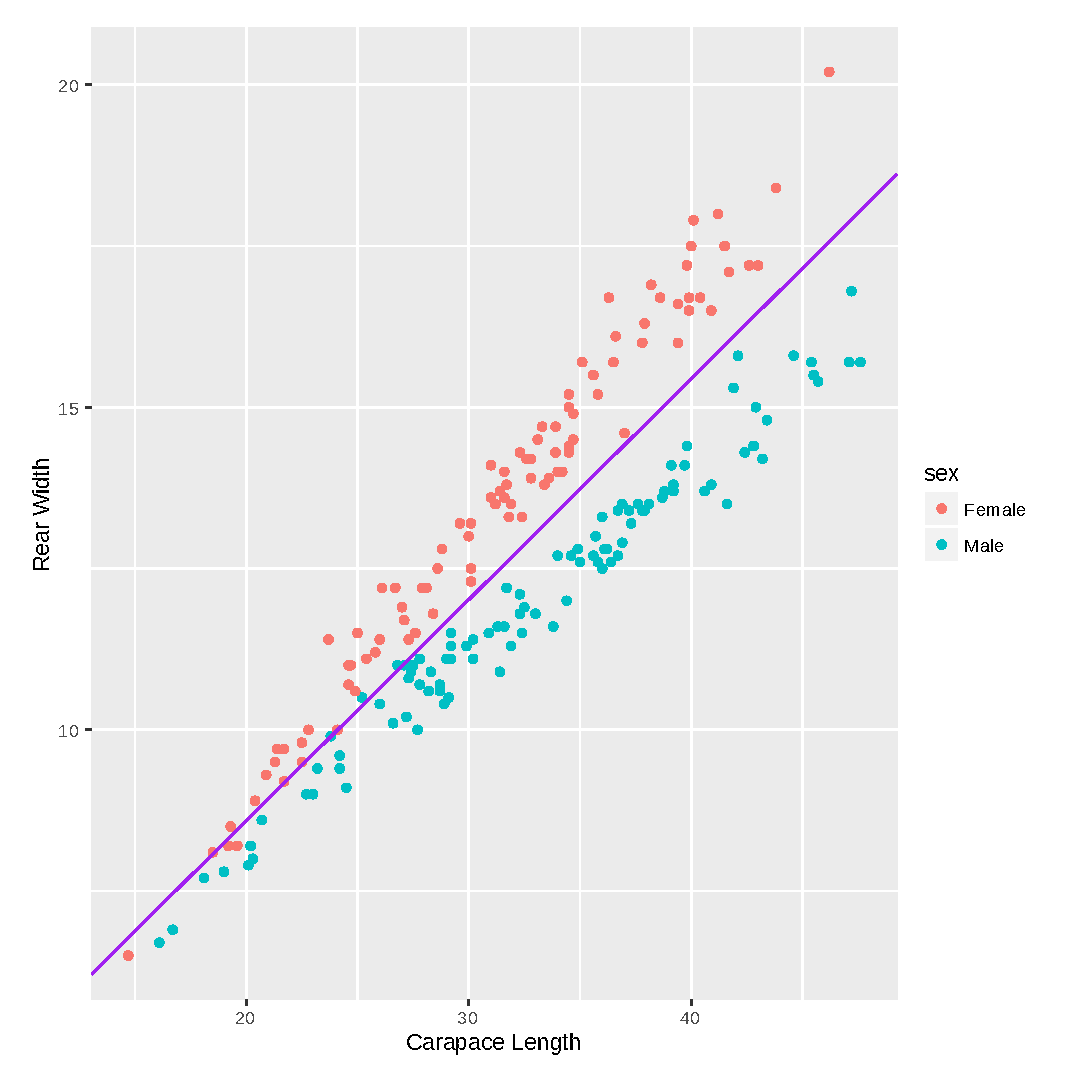
\includegraphics[width=0.44\textwidth]{share/boundarylda.eps}
        \end{figure}

        \begin{figure}[h!]
            \centering
            \caption{Crab Sex Decision Boundary using LR}
            \label{fig:boundarylr}
            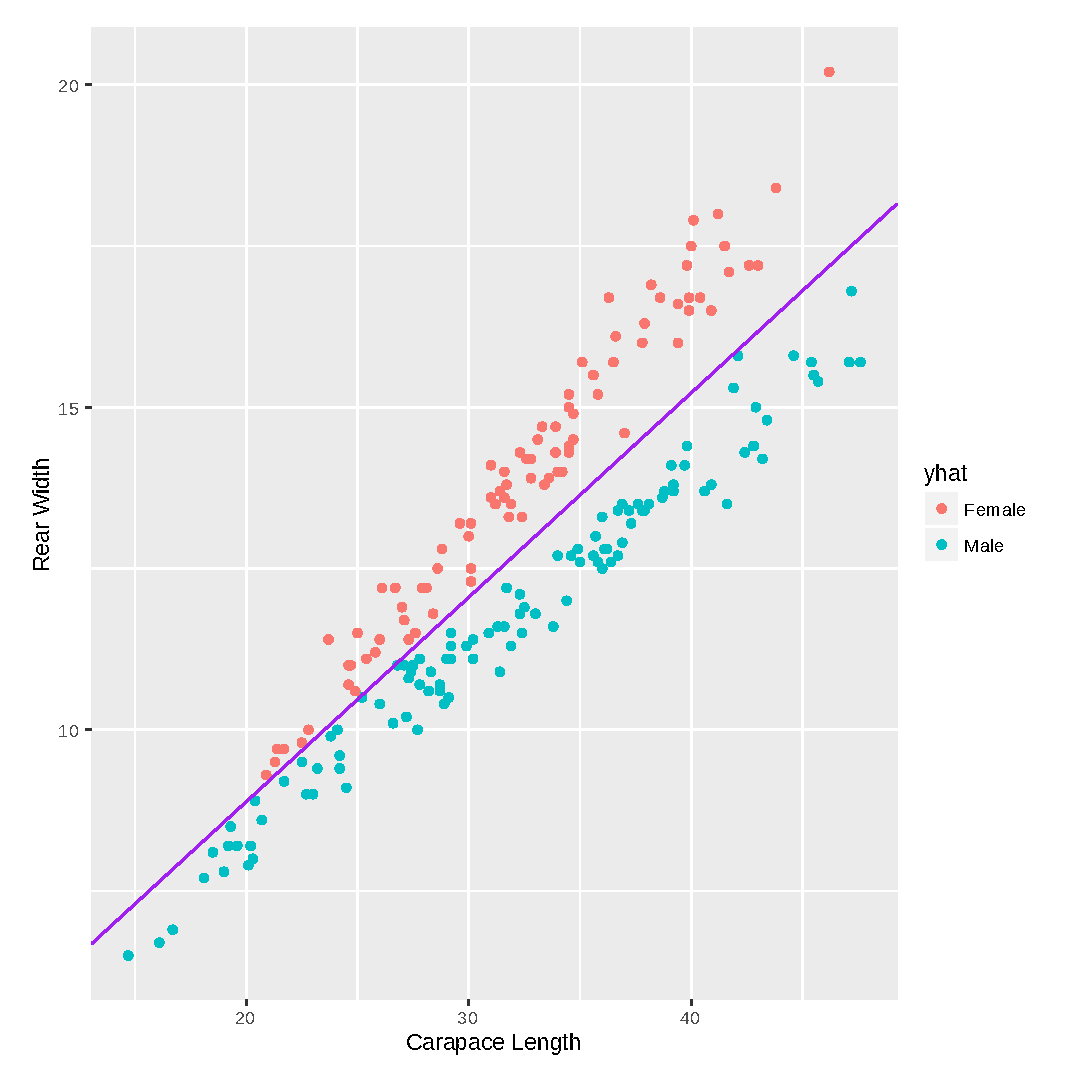
\includegraphics[width=0.44\textwidth]{share/boundarylr.eps}
        \end{figure}

        \newpage

    \section*{Assignment 2}

        Given several \emph{observations} from different \emph{customers} with certain \emph{features} and \emph{classifications} of whether they have \emph{managed their loans} \emph{good} or \emph{bad}, we are tasked to \emph{predict} if a new customer with certain set of features, will pay back their loans on time or not.

        By using \emph{decision tree learning}, which maps observations (the branches) to their conclusions (the leaves), we can predict this aforementioned model. In Listing~\ref{lst:script} under the lines \texttt{26-45}, we use \texttt{tree} to fit our model for usage on \emph{training} \& \emph{testing} sets. These models can be fit using different measures of \emph{impurity}, where we only consider \emph{deviance} and the \emph{gini index} here. In Table~\ref{table:dectree} are the results for these. It seems that \emph{gini and/or deviance} classifies better.

        \begin{table}[h!]
        \begin{center}
        \begin{tabular}{lll}
            \toprule
                \textbf{Data Set} & \textbf{Impurity Measure} & \textbf{Miss Rate} \\
            \midrule
                Training & Deviance & 0.212 \\
                Testing & Deviance & 0.236 \\
                Training & Gini & 0.230 \\
                Testing & Gini & 0.282 \\
                Training & Deviance \& Gini & 0.212 \\
                Testing & Deviance \& Gini & 0.236 \\
            \bottomrule
        \end{tabular}
        \end{center}
        \caption{Decision Tree Missclassification Rates}
        \label{table:dectree}
        \end{table}

        \begin{figure}[h!]
            \centering
            \caption{Training and Validation Deviance Values}
            \label{fig:deviance}
            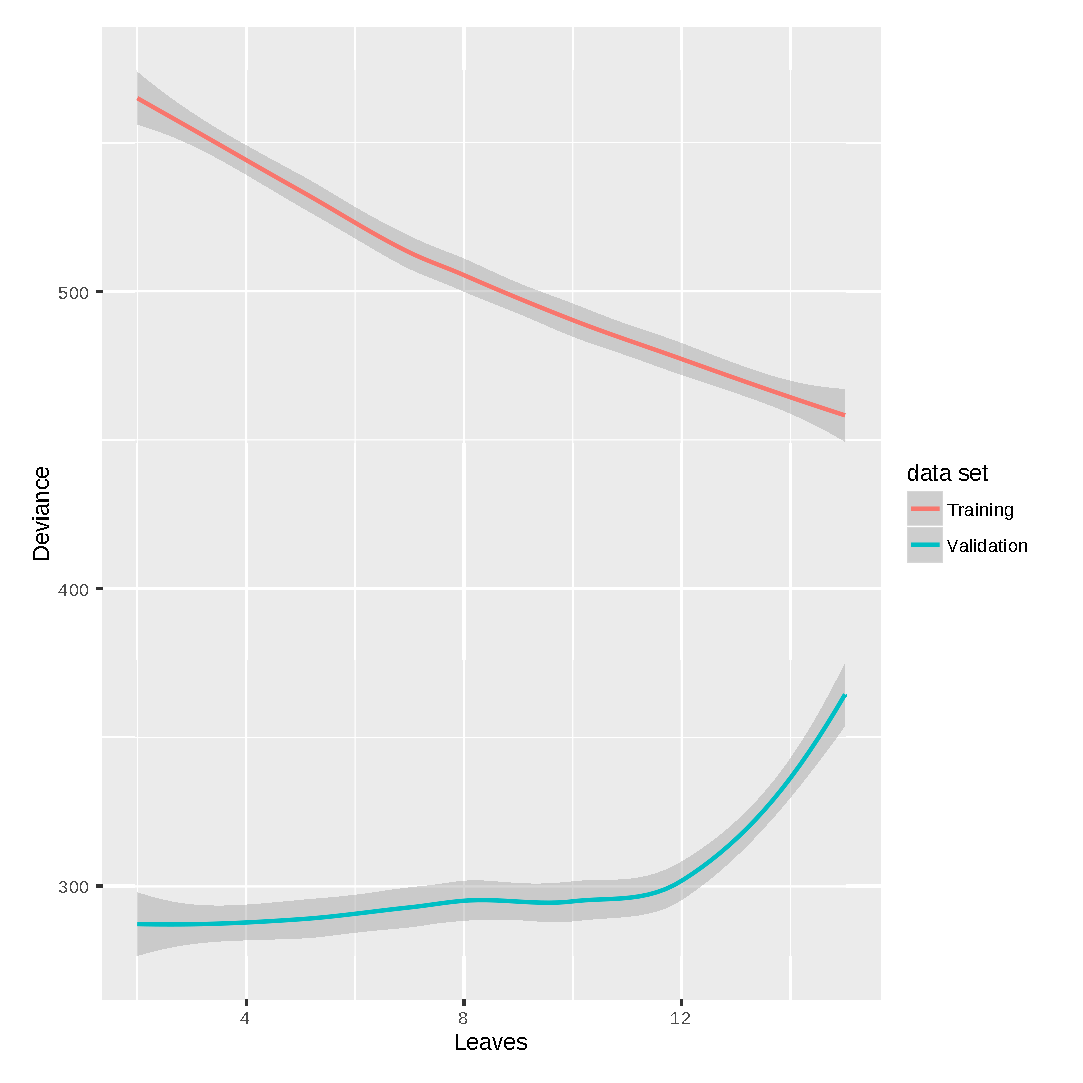
\includegraphics[width=0.5\textwidth]{share/deviance.eps}
        \end{figure}

        Afterwards, we use the \emph{training} and \emph{validation data sets} to choose the \emph{optimal tree depth}. Following lines \texttt{47-66}, we iteratively \emph{prune} the decision tree, essentially adding more \emph{leaves}, and thereafter plot the dependence on the \emph{number of leaves} and the \emph{estimated deviance of the model}. This plot can be seen in Figure~\ref{fig:deviance}. As can be seen, when more than 12 leaves are selected, the \emph{validation set} has a pretty large increase in \emph{deviance}, which isn't the desired behaviour. On the other hand, the \emph{training data set} has a constant decrease in deviance as the number of leaves increase. Therefore, the best number of leaves seems to be 12, giving best of both worlds. Additionally, the depth of this optimal tree is 6 and has a misclassification rate of 0.24 with the following features selected: \emph{savings, duration, history, age, purpose, amount, other and resident}, all of which can be found easy with \texttt{summary(tree)}.

        Finally, the decision tree is plotted in Figure~\ref{fig:tree}. Most of the branches and their outcomes seem quite reasonable (with common sense), a person that has very few savings and has a history of usually delays loans, will probably be a bad customer who doesn't pay back them. While a person which has savings and is a resident will probably be more responsible and pay back his loans. It seems that the tree has been able to select the most important features as the branches of the decision tree, which are highly correlated with either classification result (the leaves). The depth can be seen here too.

        \begin{figure}[h!]
            \centering
            \caption{Visualization of the Decision Tree}
            \label{fig:tree}
            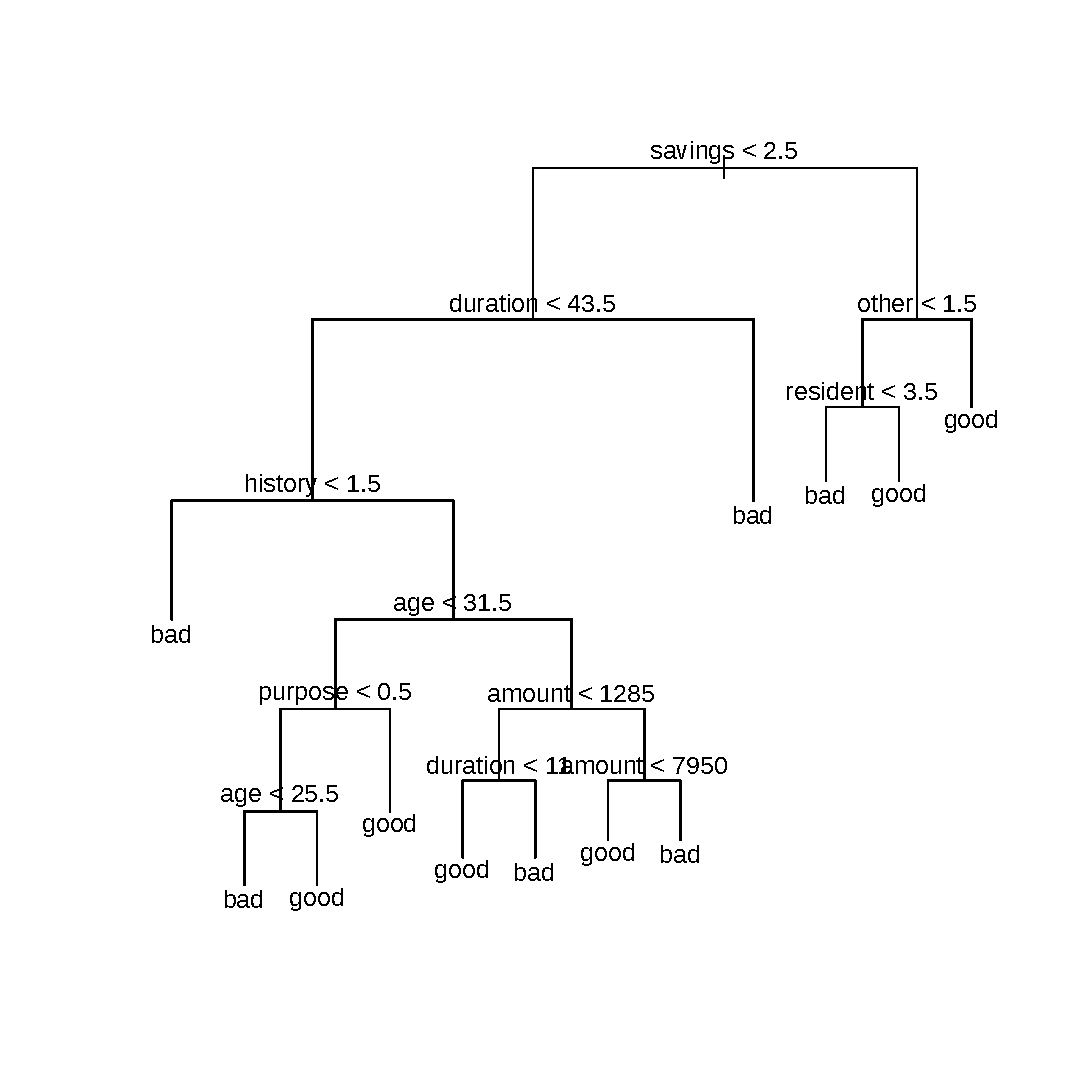
\includegraphics[width=0.45\textwidth]{share/tree.eps}
        \end{figure}

        Now we proceed to fit another model with the same situation, but using \emph{Na{\"\i}ve Bayes} instead, which basically assumes that all \emph{features} are independent, like so: $p(C_k | x_1, x_2, ..., x_n) \propto p(x_i | C_k)$.

        Under lines \texttt{82-90} we fit the model with \texttt{e1071}'s \texttt{naiveBayes} \emph{classification}, and produce the \emph{confusion matrices} and \emph{missclassifications} below for both the \emph{training} and the \emph{testing data sets}.

        \emph{Missclassification:} \emph{train} = 0.300 \& \emph{test} = 0.306.


        \begin{table}[h]
        \begin{center}
        \begin{tabular}{r|c|c|}
            \multicolumn{1}{r}{\emph{train}}
            &\multicolumn{1}{c}{\textbf{bad}}
            &\multicolumn{1}{c}{\textbf{good}} \\
            \cline{2-3}
            \textbf{bad} & 95 & 98 \\
            \cline{2-3}
            \textbf{good} & 52 & 255 \\
            \cline{2-3}
        \end{tabular}
        \begin{tabular}{r|c|c|}
            \multicolumn{1}{r}{\emph{test}}
            &\multicolumn{1}{c}{\textbf{bad}}
            &\multicolumn{1}{c}{\textbf{good}} \\
            \cline{2-3}
            \textbf{bad} & 142 & 147 \\
            \cline{2-3}
            \textbf{good} & 83 & 378 \\
            \cline{2-3}
        \end{tabular}
        \end{center}
        \caption{Normal Na{\"\i}ve Bayes Confusion Matrix}
        \label{table:bayes}
        \end{table}

        It seems that in this case, \emph{Na{\"\i}ve Bayes} performs worse than \emph{decision trees} since the missclassification rate is quite a bit higher. Now, let's assume that we are given a \emph{loss matrix}, a way of \emph{penalizing} the \emph{predictor} to apply weight to certain negatives, which in this case is $L = \left( \begin{smallmatrix}0&1\\10&0\end{smallmatrix} \right)$. Doing this in lines \texttt{92-109} results in a prediction giving the \emph{confusion matrix} below and missclassifications of train = 0.546 and test = 0.549. These missclassifications are a lot higher than those in the normal ``lossless'' model. The reason why this happens is because the cost of doing a faulty classification is highly penalized in one case (while the other isn't penalized as much), this is a underlying reason for these results.


        \begin{table}[h]
        \begin{center}
        \begin{tabular}{r|c|c|}
            \multicolumn{1}{r}{\emph{train}}
            &\multicolumn{1}{c}{\textbf{bad}}
            &\multicolumn{1}{c}{\textbf{good}} \\
            \cline{2-3}
            \textbf{bad} & 137 & 263 \\
            \cline{2-3}
            \textbf{good} & 10 & 90 \\
            \cline{2-3}
        \end{tabular}
        \begin{tabular}{r|c|c|}
            \multicolumn{1}{r}{\emph{test}}
            &\multicolumn{1}{c}{\textbf{bad}}
            &\multicolumn{1}{c}{\textbf{good}} \\
            \cline{2-3}
            \textbf{bad} & 207 & 394 \\
            \cline{2-3}
            \textbf{good} & 18 & 131 \\
            \cline{2-3}
        \end{tabular}
        \end{center}
        \caption{``Lossy'' Na{\"\i}ve Bayes Confusion Matrix}
        \label{table:bayes10}
        \end{table}

    \nocite{*}
    \bibliographystyle{alpha}
    \bibliography{report}

    \onecolumn \appendix
    \section*{Appendix}

    \lstinputlisting[caption={Linear Discriminant Analysis Assignment},label={lst:lda}]{../share/lda.r}
    \lstinputlisting[caption={Decision Trees and Na{\"\i}ve Bayes Assignment},label={lst:script}]{../share/script.r}

\end{document}
